\vspace{0.3cm}
\noindent Trong phần này, nhóm chúng em sẽ trình bày kết quả khi chạy chương trình:

\begin{figure}[H]
    \centering
    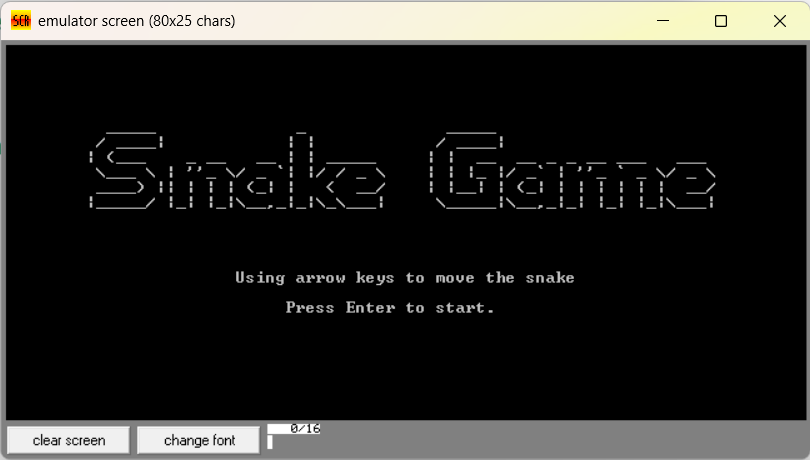
\includegraphics[width=0.85\textwidth]{Images/Game_Test/Game_test_1.png}
    \caption{Giao diện khởi đầu game}
    \label{fig:game_test_1}
\end{figure}

\noindent \textbf{Màn hình khởi đầu bao gồm:}
\begin{itemize}
    \itemsep0.2cm
    \item \textbf{Tiêu đề game:} Dòng chữ "Snake Game" được thiết kế bắt mắt.
    \item \textbf{Hướng dẫn:} Thông báo yêu cầu người chơi nhấn phím \texttt{Enter} để bắt đầu.
    \item \textbf{Tính năng:} Màn hình sẽ chuyển sang giao diện chính khi người dùng nhấn đúng phím \texttt{Enter}.
\end{itemize}

\vspace{0.5cm}
\begin{figure}[H]
    \centering
    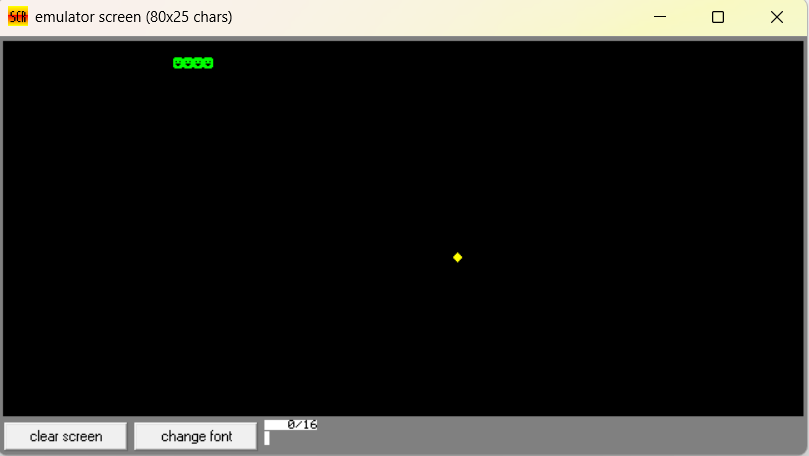
\includegraphics[width=0.85\textwidth]{Images/Game_Test/Game_test_2.png}
    \caption{Giao diện chính của game}
    \label{fig:game_test_2}
\end{figure}

\noindent \textbf{Giao diện chơi game bao gồm:}
\begin{itemize}
    \itemsep0.2cm
    \item \textbf{Con rắn:} 
    \begin{itemize}
        \item Độ dài ban đầu: 4 ô.
        \item Màu sắc mặc định: Xanh lá (\textcolor{green}{$\blacksquare$}).
    \end{itemize}
    \item \textbf{Mồi:}
    \begin{itemize}
        \item Kích thước: 1 ô.
        \item Màu sắc mặc định: Vàng (\textcolor{yellow}{$\blacksquare$}).
    \end{itemize}
    \item \textbf{Điều khiển:} Sử dụng các phím mũi tên ↑ ↓ ← → để di chuyển
\end{itemize}

\vspace{0.5cm}
\begin{figure}[H]
    \centering
    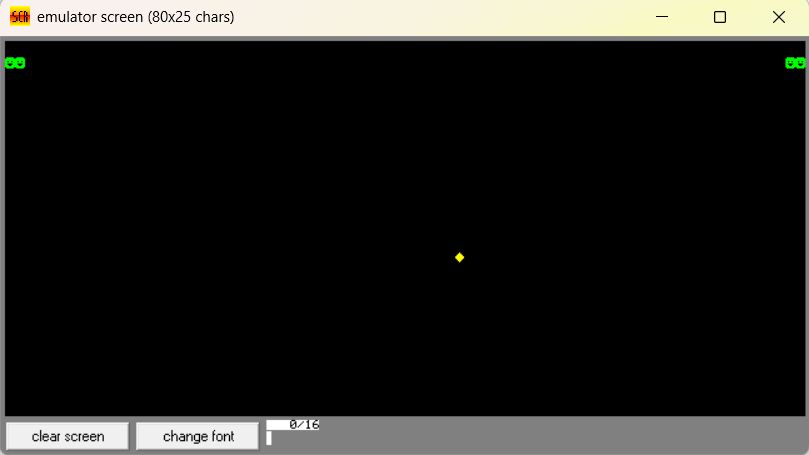
\includegraphics[width=0.85\textwidth]{Images/Game_Test/Game_test_3.png}
    \caption{Cơ chế xuyên tường}
    \label{fig:game_test_3}
\end{figure}

\noindent \textbf{Đặc điểm nổi bật:}
\begin{itemize}
    \itemsep0.2cm
    \item Khi rắn va chạm với tường, thay vì kết thúc game, rắn sẽ xuất hiện ở phía đối diện.
    \item Cơ chế này tạo độ khó vừa phải và tăng tính thú vị cho trò chơi.
\end{itemize}

\vspace{0.5cm}
\begin{figure}[H]
    \centering
    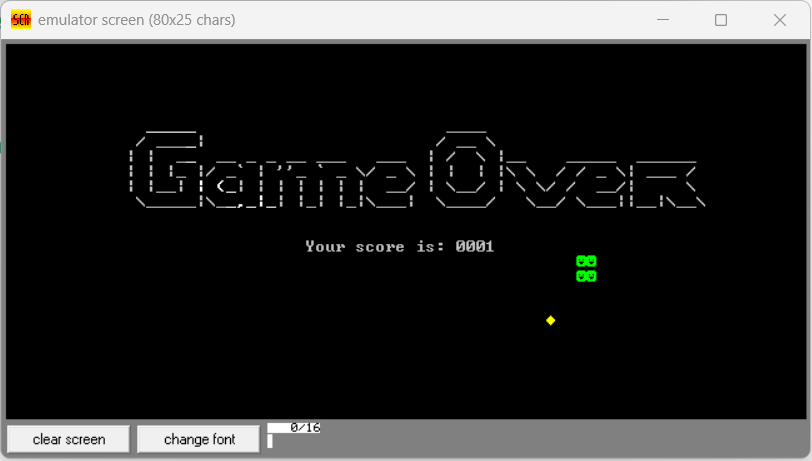
\includegraphics[width=0.85\textwidth]{Images/Game_Test/Game_test_4.png}
    \caption{Màn hình kết thúc game}
    \label{fig:game_test_4}
\end{figure}

\noindent \textbf{Màn hình kết thúc bao gồm:}
\begin{itemize}
    \itemsep0.2cm
    \item \textbf{Trạng thái cuối:} Vị trí rắn và mồi khi game kết thúc.
    \item \textbf{Thông báo:} Dòng chữ "Game Over" nổi bật.
    \item \textbf{Điểm số:} Hiển thị tổng điểm người chơi đạt được.
\end{itemize}